% D.2 一线三等角：等腰直角△ABC，∠BAC=90°，D∈BC；BE⊥AD于E，CF⊥AD于F
\documentclass[tikz,border=4pt]{standalone}
\usepackage{ctex}
\usepackage{amsmath}
\usetikzlibrary{calc}
\begin{document}
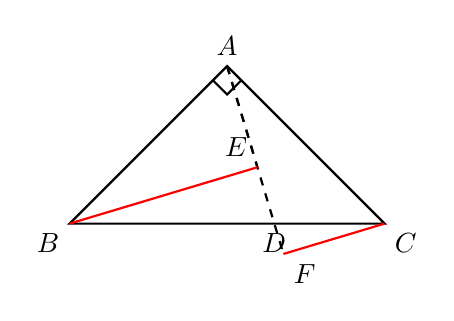
\begin{tikzpicture}[scale=1.0, thick]
  \coordinate (A) at (0, 2);
  \coordinate (B) at (-2, 0);
  \coordinate (C) at (2, 0);
  \coordinate (D) at (0.6, 0);
  % 直线 AD 方向单位向量
  \pgfmathsetmacro{\dx}{0.6-0}
  \pgfmathsetmacro{\dy}{0-2}
  \pgfmathsetmacro{\dn}{sqrt(\dx*\dx+\dy*\dy)}
  % E 在 AD 延长线上（D 之外）：B 到直线 AD 的垂足
  % 取直线 AD：参数式 (0,2)+t*(0.6,-2)，t∈R
  % B 的垂足 t = ((B-A)·v)/(v·v)，B-A=(-2,-2)，v=(0.6,-2)，v·v=4.36，dot=-1.2+4=2.8
  \pgfmathsetmacro{\tE}{((-2)*0.6 + (-2)*(-2))/(0.6*0.6 + 2*2)}
  \coordinate (E) at ({0 + \tE*0.6}, {2 + \tE*(-2)});
  % C 的垂足 t = (2*0.6 + (-2)*(-2))/4.36 = (1.2+4)/4.36
  \pgfmathsetmacro{\tF}{(2*0.6 + (-2)*(-2))/(0.6*0.6 + 2*2)}
  \coordinate (F) at ({0 + \tF*0.6}, {2 + \tF*(-2)});

  \draw (A) -- (B) -- (C) -- cycle;
  \draw[dashed] (A) -- (E);
  \draw[dashed] (A) -- (F);
  \draw[red] (B) -- (E);
  \draw[red] (C) -- (F);

  % 直角符号 at A
  \draw ($(A)+(-0.18,-0.18)$) -- ($(A)+(0,-0.36)$) -- ($(A)+(0.18,-0.18)$);

  \node[above]       at (A) {$A$};
  \node[below left]  at (B) {$B$};
  \node[below right] at (C) {$C$};
  \node[below]       at (D) {$D$};
  \node[above left]  at (E) {$E$};
  \node[below right] at (F) {$F$};
\end{tikzpicture}
\end{document}
